\documentclass[Arkitektur/System_main.tex]{subfiles}
\begin{document}

\subsection{Sekvensdiagram for UC3 End game} \label{sec:ssd_UC3}
End game sekvens skal læses som, det sekvens der køres når et hold har tabt. I sekvensdiagrammet for UC3 End game antages der, at Opponent Team taber spillet på Playerside 2, men det behøver ikke at være Playerside 2. Man kan i denne tilfælde godt bytte rundt med Playerside 1 og 2 uden at det påvirker sekvensdiagrammet.
\begin{figure}
    \centering 
    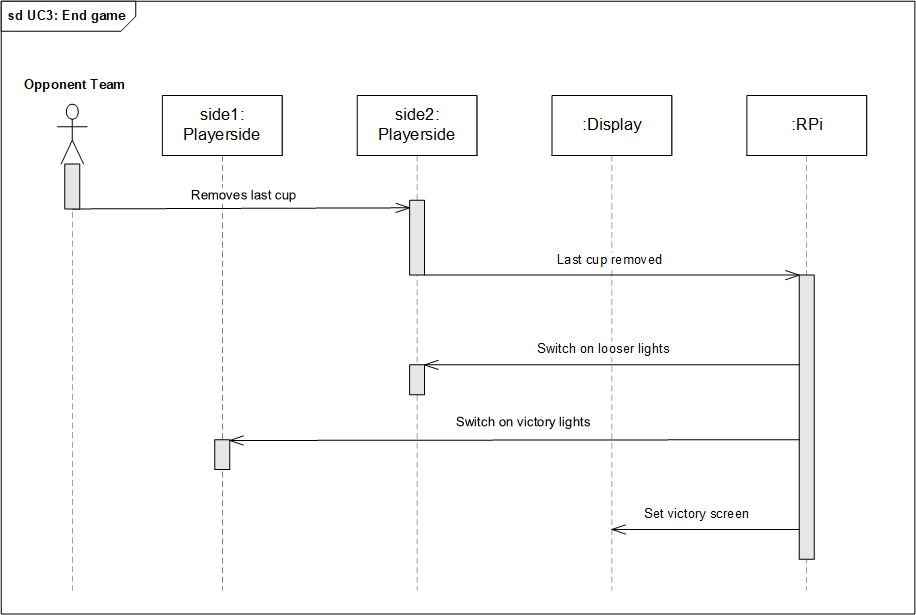
\includegraphics[width=\linewidth]{Arkitektur/Sekvensdiagrammer/graphics/sd_UC3.png}
    \caption{Sekvensdiagram for UC3 - End Game}
    \label{fig:sd_UC3}
\end{figure}
\newpage
\end{document}